% Gemini theme
% https://github.com/anishathalye/gemini

\documentclass[final]{beamer}

% ====================
% Packages
% ====================

\usepackage[T1]{fontenc}
\usepackage{lmodern}

% set poster dimensions below (in cm)
% ACIC poster max size is 42" x 42", or 106.68 cm x 106.68 cm
% for a 16/9 aspect ratio, using 
\usepackage[size=custom,width=100,height=56.25,scale=0.85]{beamerposter}
\usetheme{gemini}
\usecolortheme{mit}
\usepackage{graphicx}
\usepackage{booktabs}

% \usepackage{amsmath}
% \usepackage{amsfonts}
% \usepackage{amsthm}
\usepackage{tikz}
\usepackage{subcaption}
\usepackage{pgfplots}
\pgfplotsset{compat=1.14}
\usepackage{anyfontsize}
\usepackage{hyperref}

\usepackage{hayesmacros}


% \theoremstyle{definition}
% \newtheorem{definition}{Definition}
% \newtheorem{assumption}{Assumption}
% \newtheorem{example}{Example}

% \theoremstyle{plain}
% \newtheorem{proposition}{Proposition}
% \newtheorem{lemma}{Lemma}
% \newtheorem{theorem}{Theorem}
% \newtheorem{corollary}{Corollary}

% \theoremstyle{remark}
% \newtheorem{remark}{Remark}

\hypersetup{colorlinks,allcolors=blue}
\geometry{left=1in,right=1in,top=1in,bottom=1in}

% ====================
% Lengths
% ====================

% If you have N columns, choose \sepwidth and \colwidth such that
% (N+1)*\sepwidth + N*\colwidth = \paperwidth
\newlength{\sepwidth}
\newlength{\colwidth}
\setlength{\sepwidth}{0.025\paperwidth}
\setlength{\colwidth}{0.3\paperwidth}

\newcommand{\separatorcolumn}{\begin{column}{\sepwidth}\end{column}}

% ====================
% Title
% ====================

\title{Estimating network-mediated causal effects via spectral embeddings}

\author{Alex Hayes \inst{1} \and Mark M. Fredrickson \inst{2} \and Keith Levin \inst{1}}

\institute[shortinst]{\inst{1} Department of Statistics, University of Wisconsin-Madison \samelineand \inst{2} Department of Statistics, University of Michigan}

% ====================
% Footer (optional)
% ====================

\footercontent{
  \href{https://www.alexpghayes.com}{https://www.alexpghayes.com} \hfill
  % \href{https://www.alexpghayes.com}{https://www.alexpghayes.com} \hfill
  ACIC 2023, Austin, TX \hfill
  \href{mailto:alex.hayes@wisc.edu}{alex.hayes@wisc.edu}}
% (can be left out to remove footer)

% ====================
% Logo (optional)
% ====================

% use this to include logos on the left and/or right side of the header:
\logoright{
\includegraphics[height=7cm]{figures/logos/color-flush-UWlogo-print.pdf}}
\logoleft{
\includegraphics[scale=1.5]{figures/logos/U-M_Logo-Horizontal-Hex.png}}

% ====================
% Body
% ====================

\begin{document}

\begin{frame}[t]
  \begin{columns}[t]
    \separatorcolumn

    \begin{column}{\colwidth}

      \begin{alertblock}{Abstract}

        We consider the task of mediation analysis for network data, and present a model in which mediation occurs in a latent embedding space. Under this model, node-level interventions have causal effects on nodal outcomes, and these effects can be partitioned into a direct effect independent of the network, and an indirect effect induced by homophily.

      \end{alertblock}

      \begin{block}{Motivating example: smoking in adolescent social networks}

        \begin{figure}[ht!]
          \begin{subfigure}{0.49\textwidth}
            \centering
            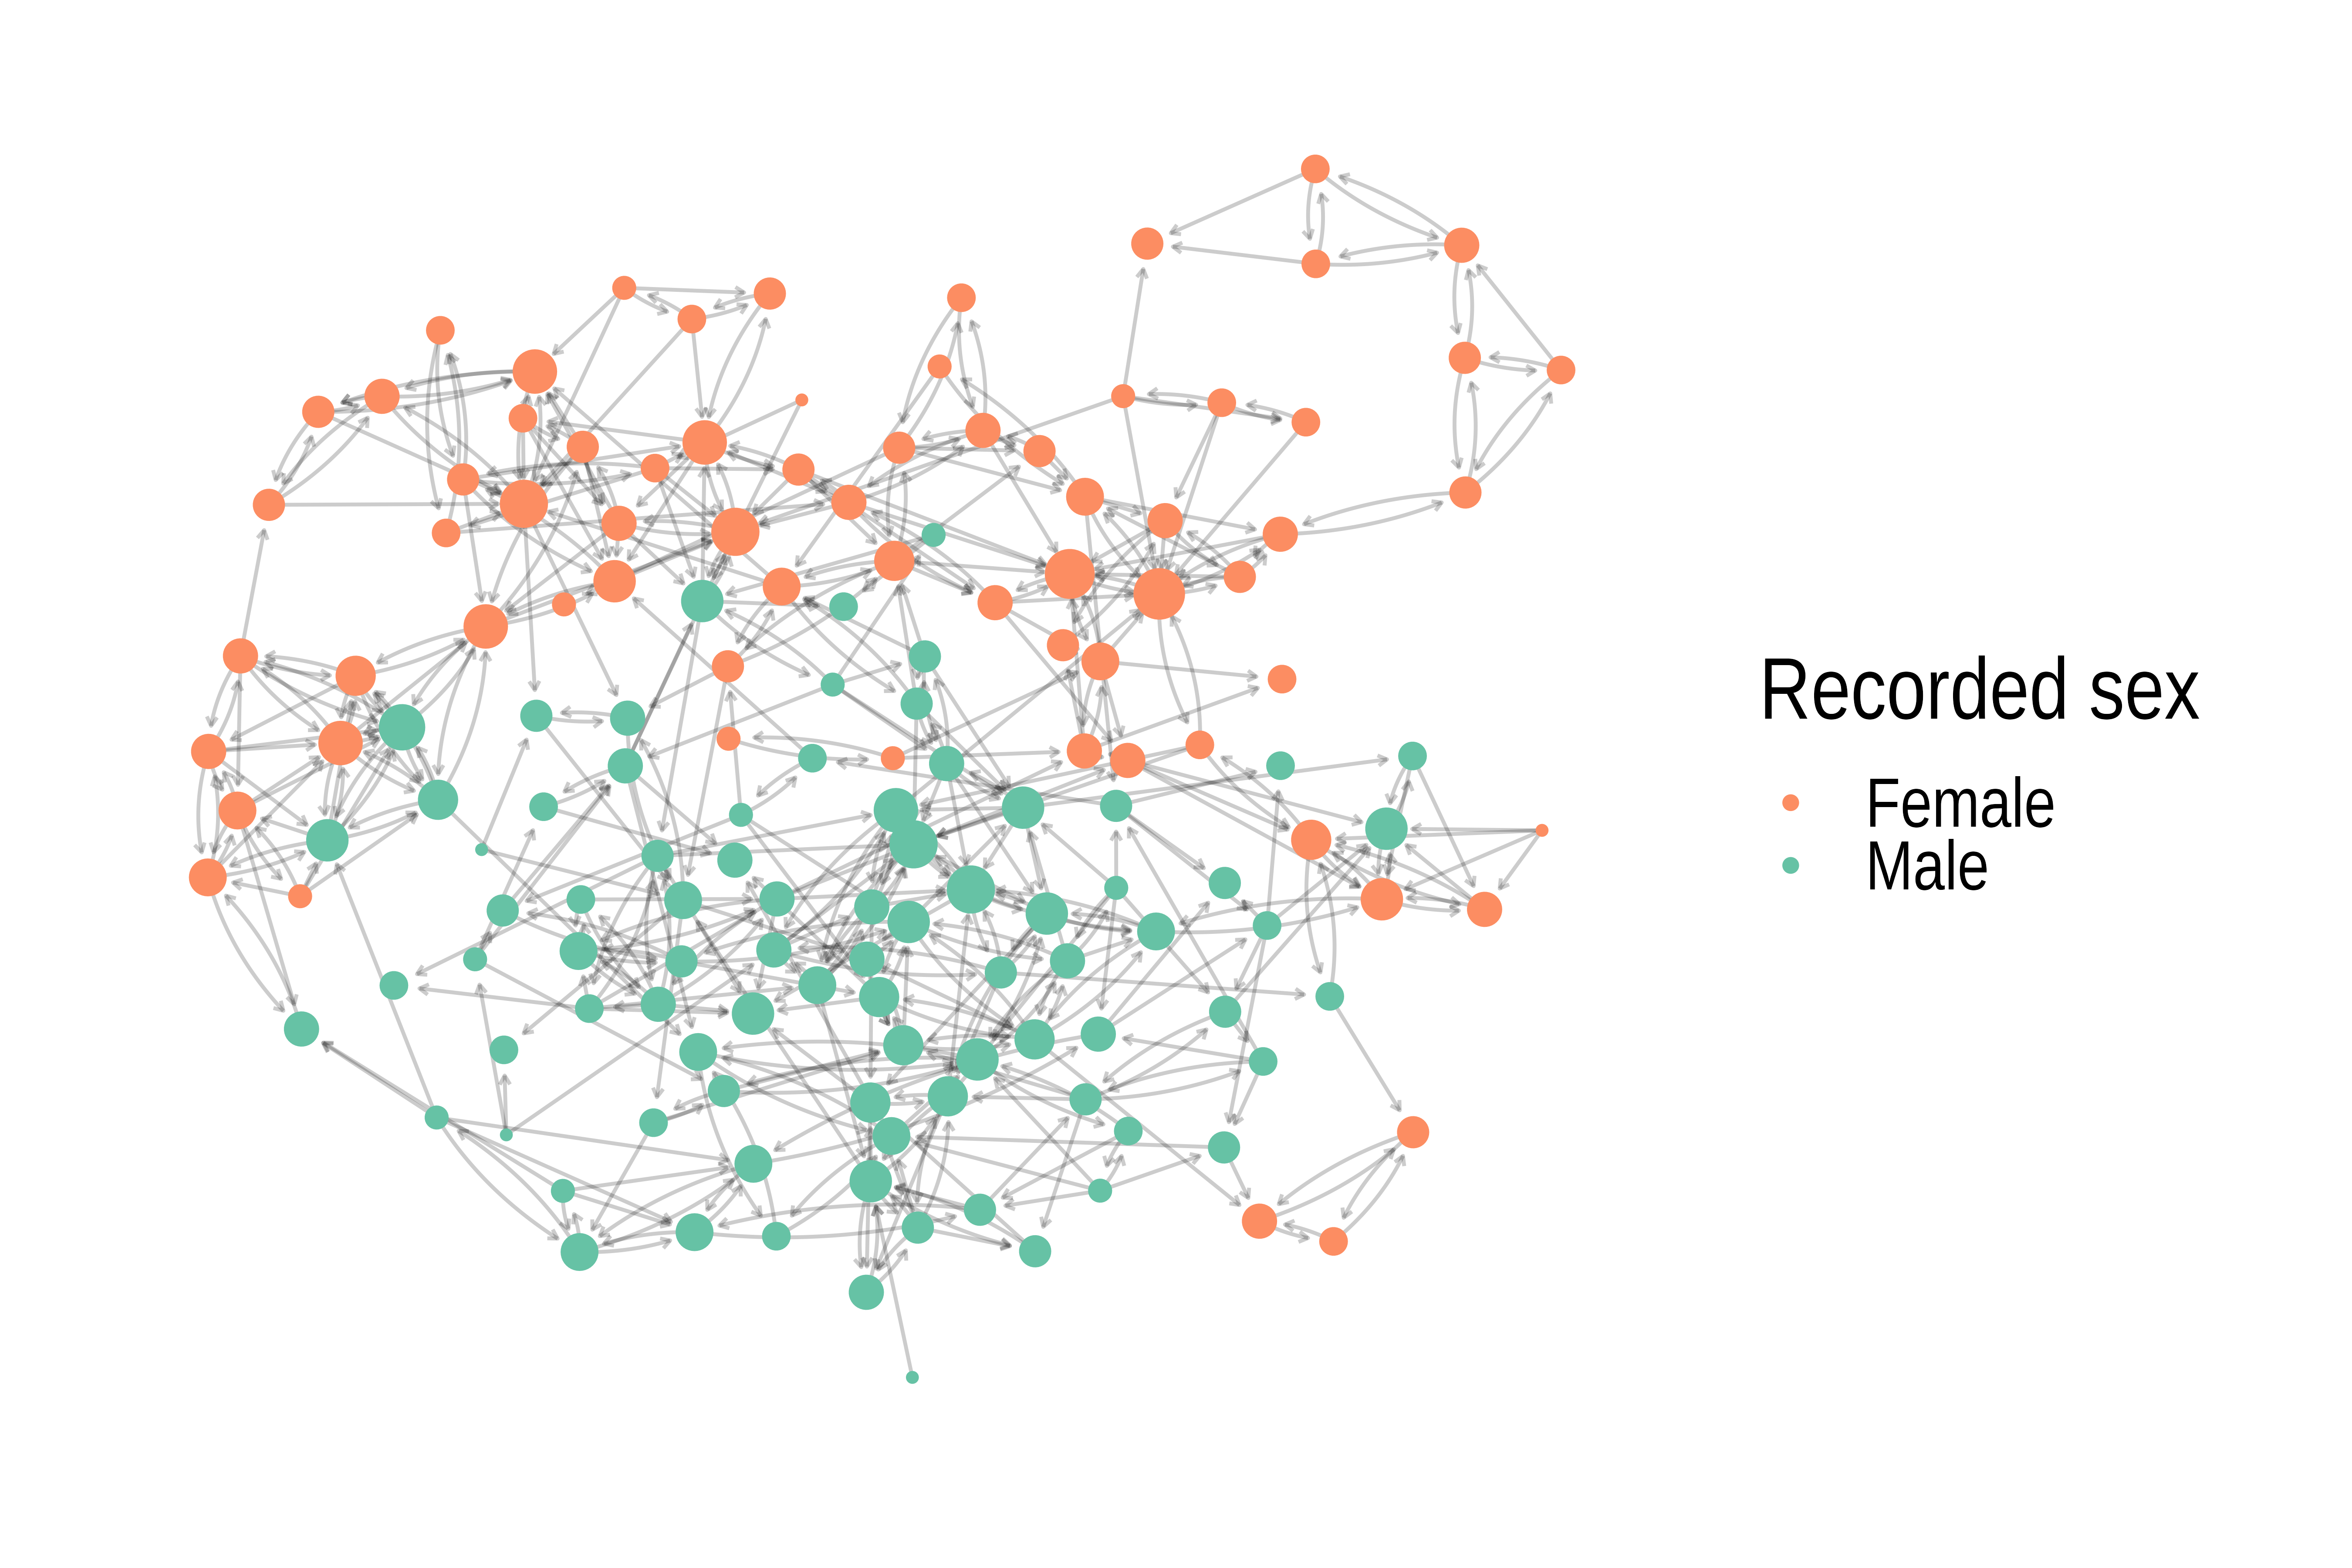
\includegraphics[width=\textwidth]{figures/glasgow/sex.png}
          \end{subfigure}
          \begin{subfigure}{0.49\textwidth}
            \centering
            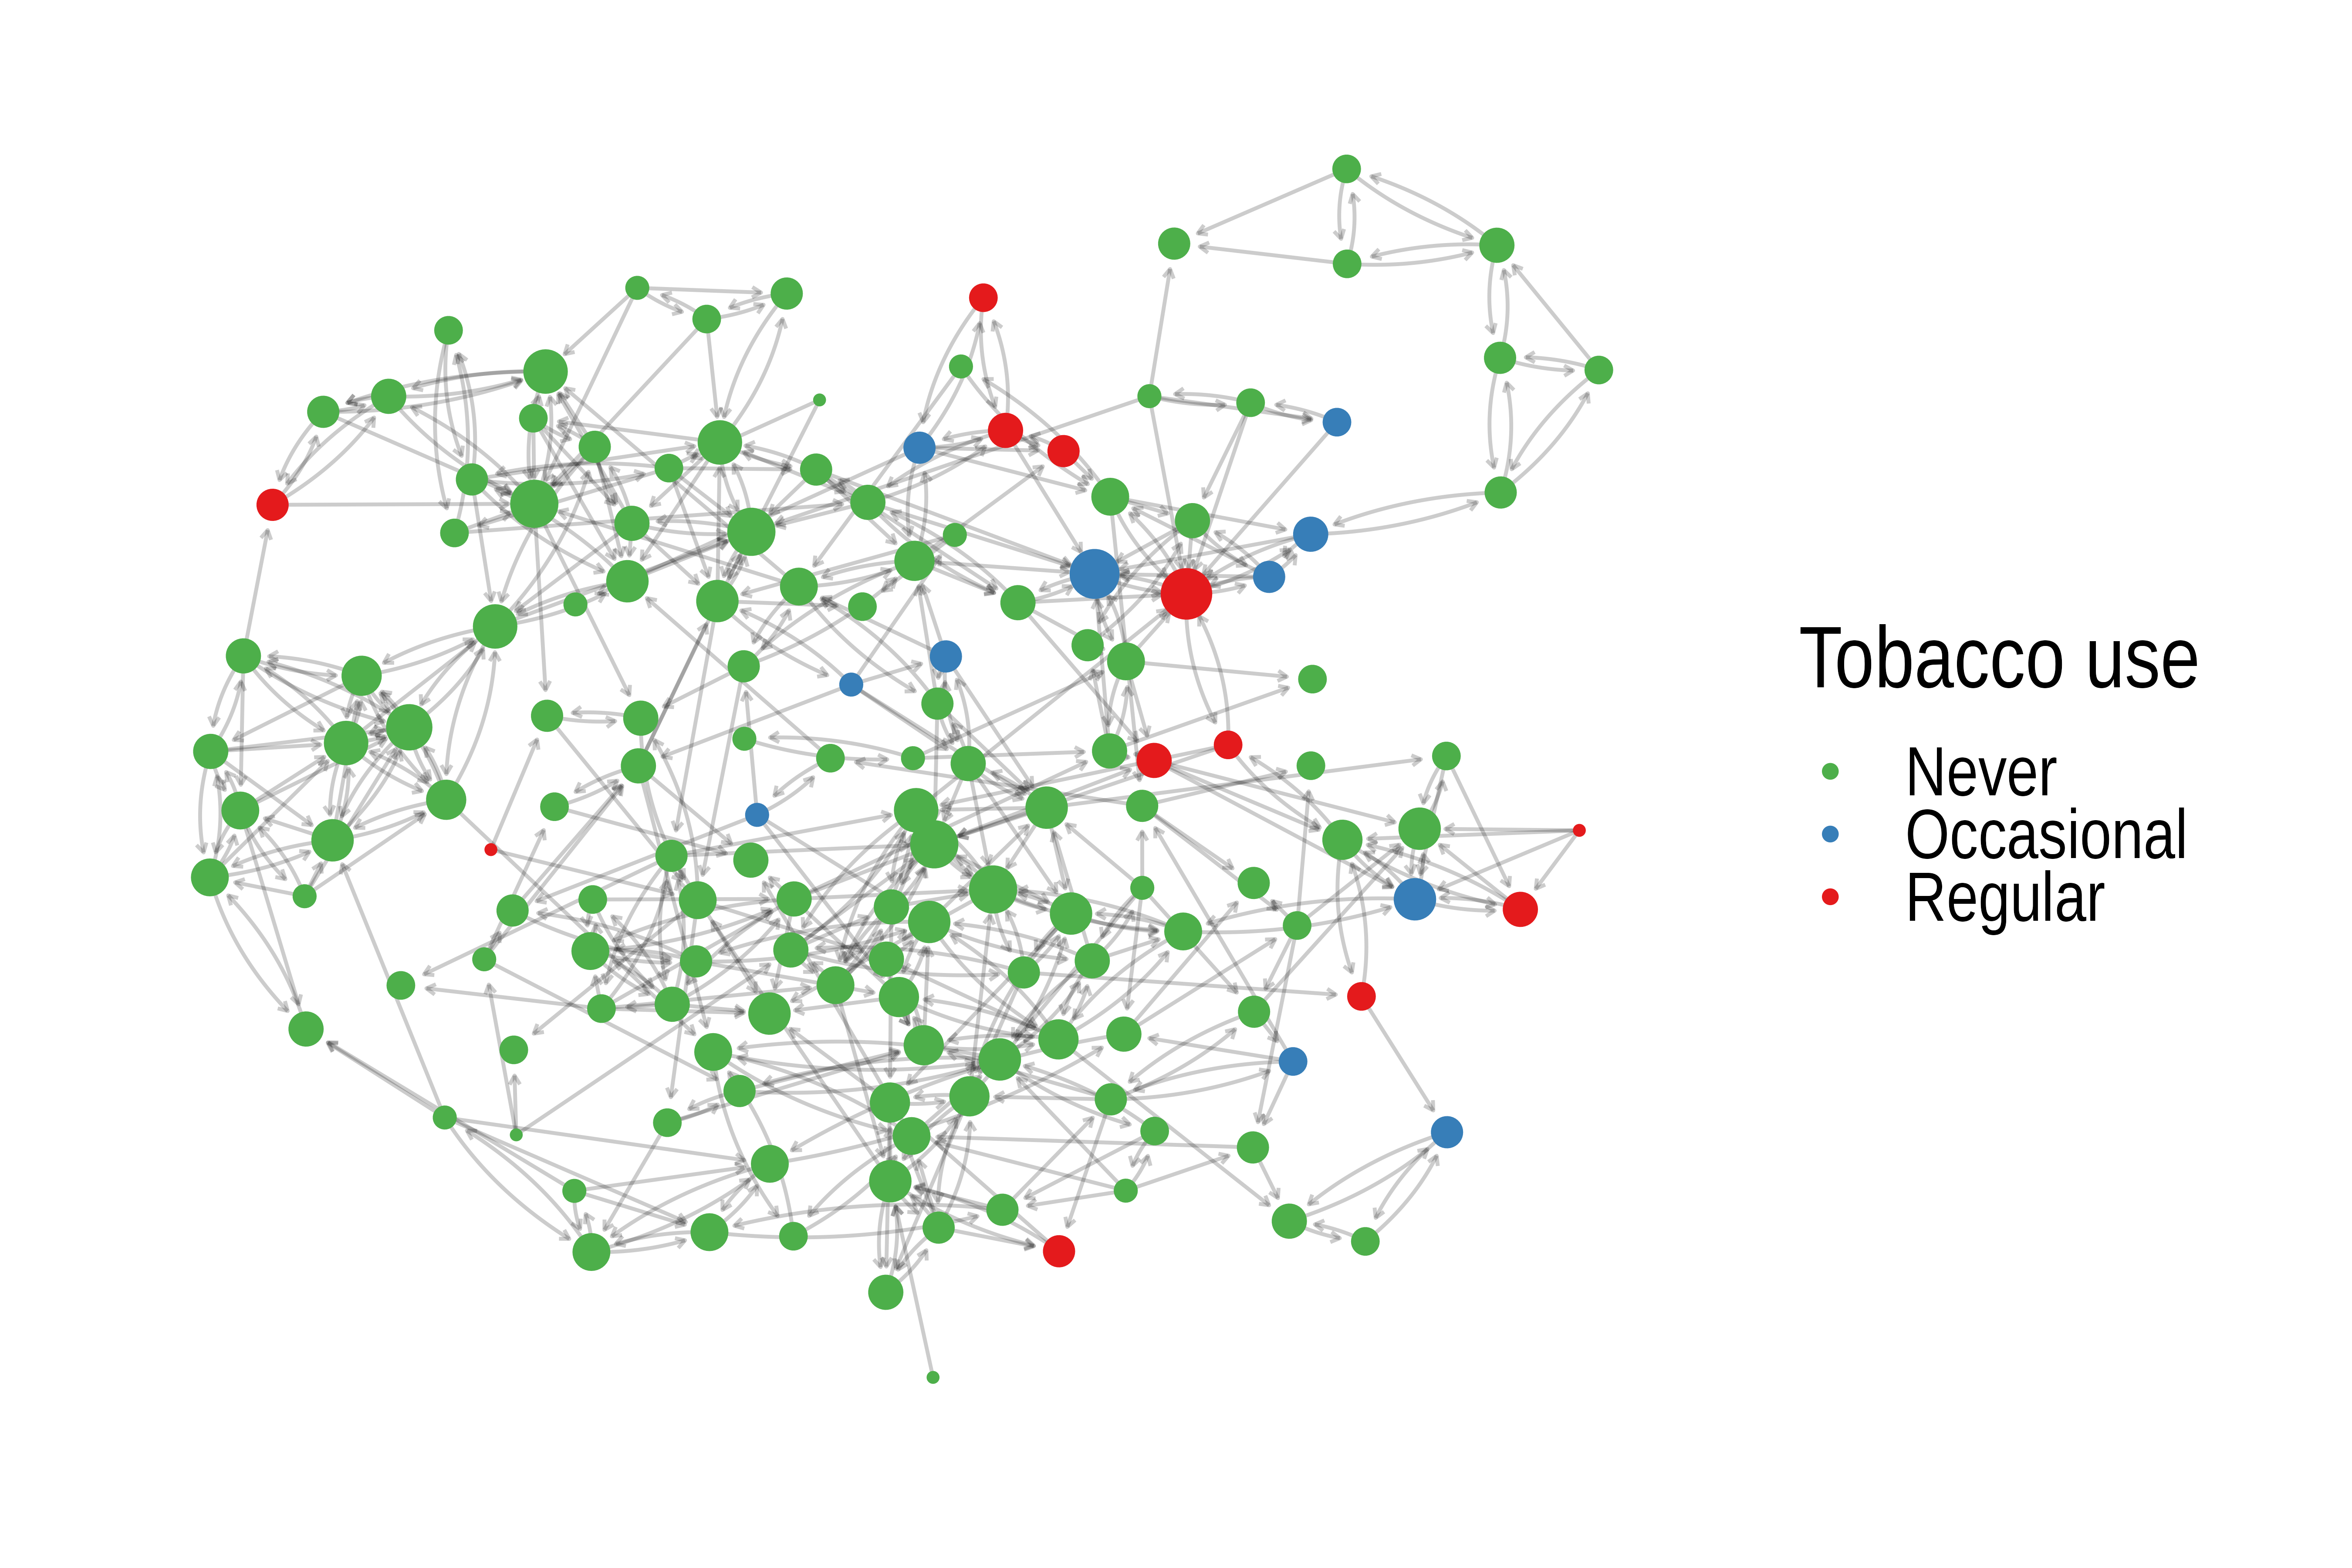
\includegraphics[width=\textwidth]{figures/glasgow/tobacco.png}
          \end{subfigure}
          \caption{Directed friendships in a secondary school in Glasgow, reported in the Teenage Friends and Lifestyle Study (wave 1). Each node represents one student.}
          \label{fig:glasgow}
        \end{figure}

      \end{block}


      \begin{block}{Notation \& inferential targets}

        \begin{minipage}{.5\textwidth}

          \centering

          We assume we have a (symmetric) network with nodes $1, ..., n$.

          \vspace{1cm}

          \begin{table}[]
            \begin{tabular}{lcc}
              Network adjacency matrix & $A$            & $\in \R^{n \times n}$ \\
              Edge $i \sim j$          & $A_{ij}$       & $\in \R$              \\
              Treatment                & $T_i$          & $\in \set{0, 1} $     \\
              Outcome                  & $Y_i$          & $\in \R$              \\
              Confounders              & $\C_{i \cdot}$ & $\in \R^p$            \\
              Friend group (latent)    & $\X_{i \cdot}$ & $\in \R^d$
            \end{tabular}
          \end{table}

        \end{minipage}
        \begin{minipage}{.5\textwidth}

          \begin{figure}[ht]
            \centering
            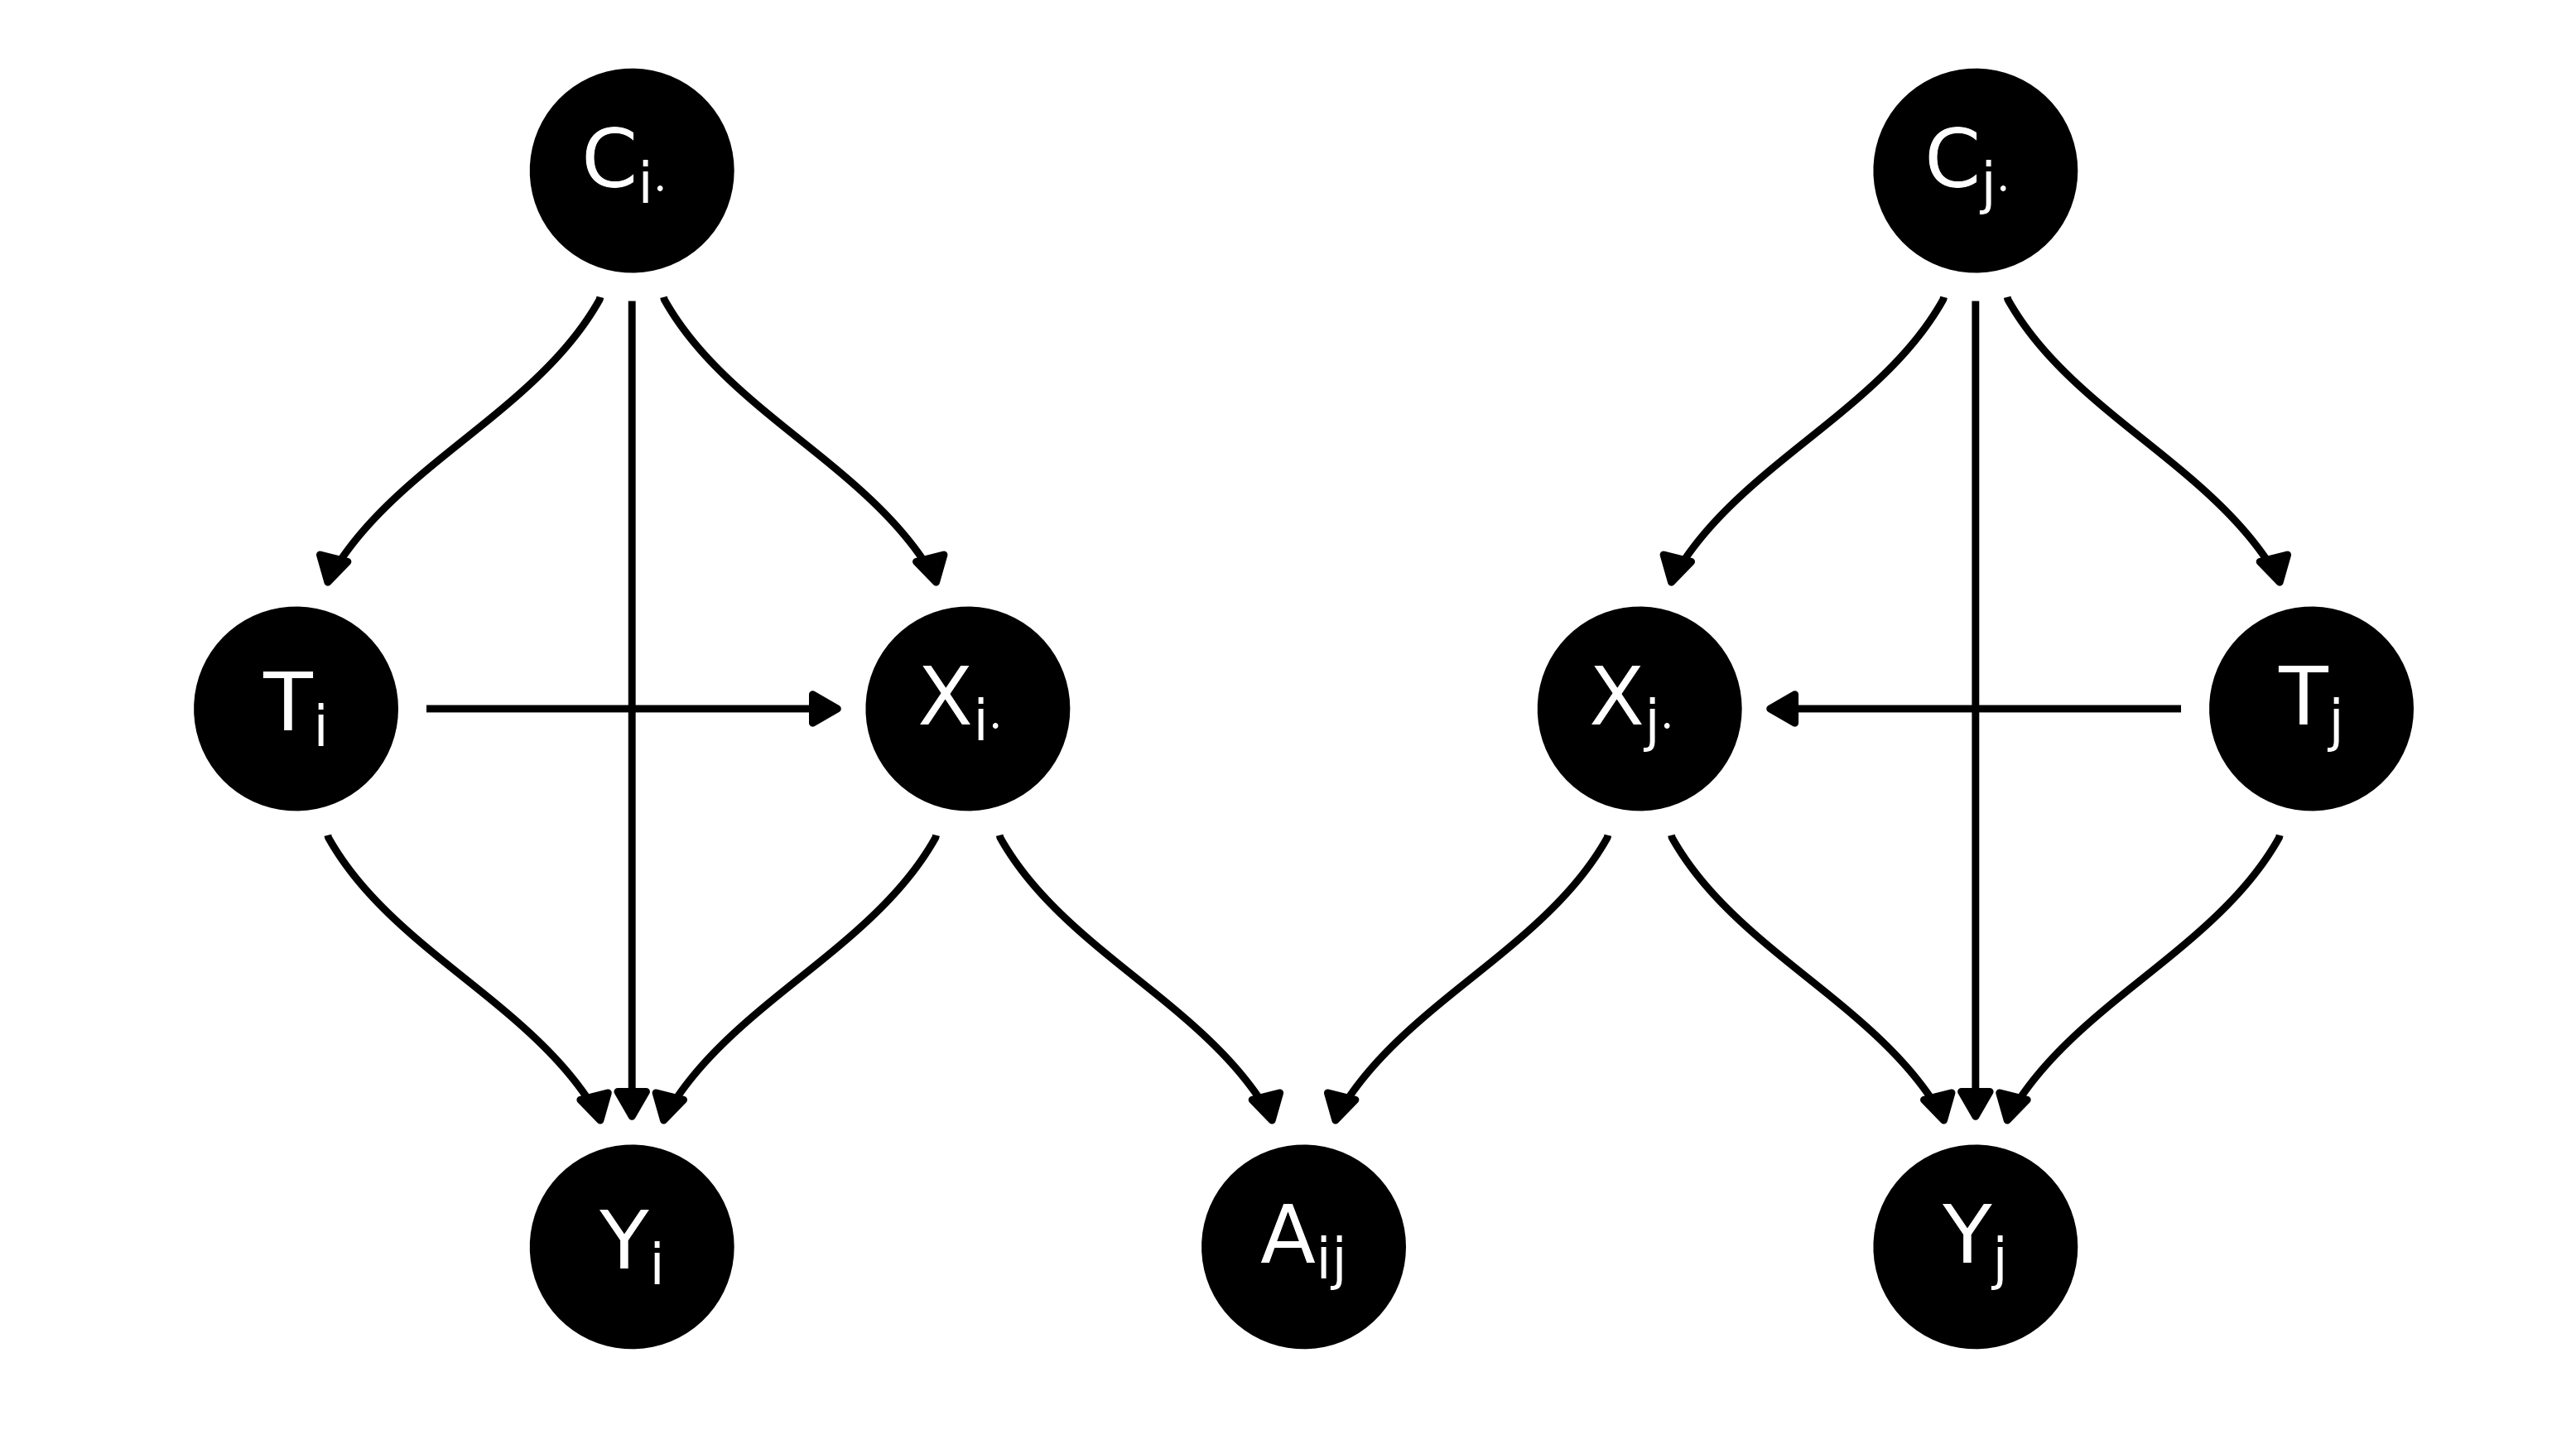
\includegraphics[width=\textwidth]{figures/dags/full_mediating.png}
            \caption{A directed acyclic graph (DAG) representing the causal pathways in a network with homophilous mediation, for node a network with two nodes called $i$ and $j$.}
            \label{fig:mediating}
          \end{figure}

        \end{minipage}

        We are interested in the causal effect of $T_i$ on $Y_i$ as mediated by the latent position $\X_{i \cdot}$. More precisely, we want to estimate the \emph{natural direct effect} and the \emph{natural indirect effect}
        \begin{align*}
          \ndef & = \E{Y_i(t, \X_{i \cdot}(t^*)) - Y_i(t^*, \X_{i \cdot}(t^*))} \\
          \nief & = \E{Y_i(t, \X_{i \cdot}(t)) - Y_i(t, \X_{i \cdot}(t^*))}
        \end{align*}
      \end{block}

    \end{column}

    \separatorcolumn

    \begin{column}{\colwidth}

      \begin{block}{Semi-parametric network model}

        Let $A \in \R^{n \times n}$ be a random symmetric matrix, such as the adjacency matrix of an undirected graph. Let $\Apop = \E[\X]{A} = \X \X^T$ be the expectation of $A$ conditional on $\X \in \R^{n \times d}$, which has independent and identically distributed rows $\X_{1 \cdot}, \dots, \X_{n \cdot}$. That is, $\Apop$ has $\rank \paren*{\Apop} = d$ and is positive semi-definite with eigenvalues $\lambda_1 \ge \lambda_2 \ge \cdots \ge \lambda_d > 0 = \lambda_{d+1} = \cdots = \lambda_n$. Conditional on $\X$, the upper-triangular elements of $A - \Apop$ are independent $(\nu_n, b_n)$-sub-gamma random variables.

        Examples: (degree-corrected) stochastic blockmodels, mixed-membership blockmodels, overlapping blockmodels, (weighted, noisily-observed) random dot product graphs, LDA, factor models, etc

        The outcome regression functional is linear in $T_i, \C_{i \cdot}$, and $\X_{i \cdot}$ and the mediator regression functional is linear in $T_i, \C_{i \cdot}$, and $T_i \cdot \C_{i \cdot}$:

        \begin{equation*}
          \begin{aligned}
            \underbrace{\E[T_i, \C_{i \cdot}, \X_{i \cdot}]{Y_i}}_{\R}
             & = \underbrace{\betazero}_{\R}
            + \underbrace{T_i}_{\{0, 1\}} \underbrace{\betat}_{\R}
            + \underbrace{\C_{i \cdot}}_{\R^{1 \times p}} \underbrace{\betac}_{\R^{p}}
            + \underbrace{\X_{i \cdot}}_{\R^{1 \times d}} \underbrace{\betax}_{\R^d},
             & \text{(outcome model)}                      \\
            \underbrace{\E[T_i, \C_{i \cdot}]{\X_{i \cdot}}}_{\R^{1 \times d}}
             & = \underbrace{\thetazero}_{\R^{1 \times d}}
            + \underbrace{T_i}_{\{0, 1\}} \underbrace{\thetat}_{\R^{1 \times d}}
            + \underbrace{\C_{i \cdot}}_{\R^{1 \times p}} \underbrace{\Thetac}_{\R^{p \times d}}
            + \underbrace{T_i}_{\{0, 1\}} \underbrace{\C_{i \cdot}}_{\R^{1 \times p}} \underbrace{\Thetatc}_{\R^{p \times d}}.
             & \text{(mediator model)}
          \end{aligned}
        \end{equation*}

        Under these moment assumptions, and DAG of Figure \ref{fig:mediating}, letting $\mu_c$ denote the mean of $\C_{i \cdot}$, we have the following identification result:
        \begin{align*}
          \ndef & = \paren*{t - t^*} \, \betat, ~ \text{ and }                                        \\
          \nief & = \paren*{t - t^*} \, \thetat \, \betax + (t - t^*) \, \mu_c \, \Thetatc \, \betax.
        \end{align*}
      \end{block}

      \begin{block}{Estimation challenge: friend groups $\X$ unknown!}

        The \emph{adjacency spectral embedding} (ASE) of $A$ is well-known to be a good estimate of $\X$ under a broad, semi-parametric class of network models. Given a network with adjacency matrix $A$, the $d$-dimensional ASE is defined as
        \begin{equation*}
          \Xhat = \Uhat \Shat^{1/2} \in \R^{n \times d},
        \end{equation*}
        where $\Uhat \Shat \Uhat^T$ is the rank-$d$ truncated singular value decomposition of $A$. Under a suitably well-behaved network model, if $d$ is correctly specified or consistently estimated, there is some $d \times d$ orthogonal matrix $Q$ such that
        \begin{equation*}
          \max_{i \in [n]} \, \norm*{\Xhat_{i \cdot} - \X_{i \cdot} Q} = \op{1}.
        \end{equation*}
      \end{block}


    \end{column}

    \separatorcolumn

    \begin{column}{\colwidth}

      \begin{block}{Estimation: plug in $\Xhat$ for $\X$}
        Let $\Dhat = \begin{bmatrix} 1 & T & \C& \Xhat \end{bmatrix} \in \R^{n \times (2 + p + d)}$ and $\Wfull = \begin{bmatrix} 1 & T & \C & T \cdot \C \end{bmatrix} \in \R^{n \times (2 p + 2)}$. We estimate $\betaw$ and $\betax$ via ordinary least squares as follows
        \begin{equation*}
          \begin{bmatrix}
            \betawhat \\
            \betaxhat
          \end{bmatrix}
          = \paren*{\Dhat^T \Dhat}^{-1} \Dhat^T Y.
        \end{equation*}

        Similarly, we estimate $\Theta$ via ordinary least squares as
        \begin{equation*}
          \Thetahat
          = \paren*{\Wfull^T \Wfull}^{-1} \Wfull^T \Xhat.
        \end{equation*}

        To estimate $\nde$ and $\nie$, we combine regression coefficients from the network regression models
        \begin{align*}
          \cdehat & = \ndehat = \paren*{t - t^*} \, \betathat                                                                              & \text{and} \\
          \niehat & = \paren*{t - t^*} \, \thetathat \, \betaxhat + \paren*{t - t^*} \cdot \widehat{\mu}_c \cdot \Thetatchat \, \betaxhat,
        \end{align*}
        where $\widehat{\mu}_c$ is the sample mean of $\C_{i \cdot}$.
      \end{block}

      \begin{exampleblock}{Theory}

        Under a suitable network model and moment bounds on the regression errors, there exists a sequence of orthogonal matrices $\set{Q_n}_{n=1}^\infty$ such that

        \begin{equation*}
          \begin{aligned}
            \sqrt{ n } \,
            \Sigmahattheta^{-1/2}
            \begin{pmatrix}
              \vecc \paren*{\Thetahat \, Q_n^T} - \Thetavec
            \end{pmatrix}
             & \to
            \Normal{0}{I_{p d}}, \text{ and } \\
            \sqrt{ n } \,
            \Sigmahatbeta^{-1/2}
            \begin{pmatrix}
              \betawhat - \betaw \\
              Q_n \, \betaxhat - \betax
            \end{pmatrix}
             & \to
            \Normal{0}{I_d}.
          \end{aligned}
        \end{equation*}
        Further,
        \begin{align*}
          \sqrt{n \, \sigmahatnde} \paren*{\ndehat - \nde}
           & \to
          \Normal{0}{1}, \text{and} \\
          \sqrt{n \, \sigmahatnie} \paren*{\niehat - \nie}
           & \to
          \Normal{0}{1},
        \end{align*}
        where $\sigmahatnde$ and $\sigmahatnie$ are derived via the Delta method.

      \end{exampleblock}

      \begin{block}{Results applied to Glasgow data}

        \begin{figure}[ht!]
          \centering
          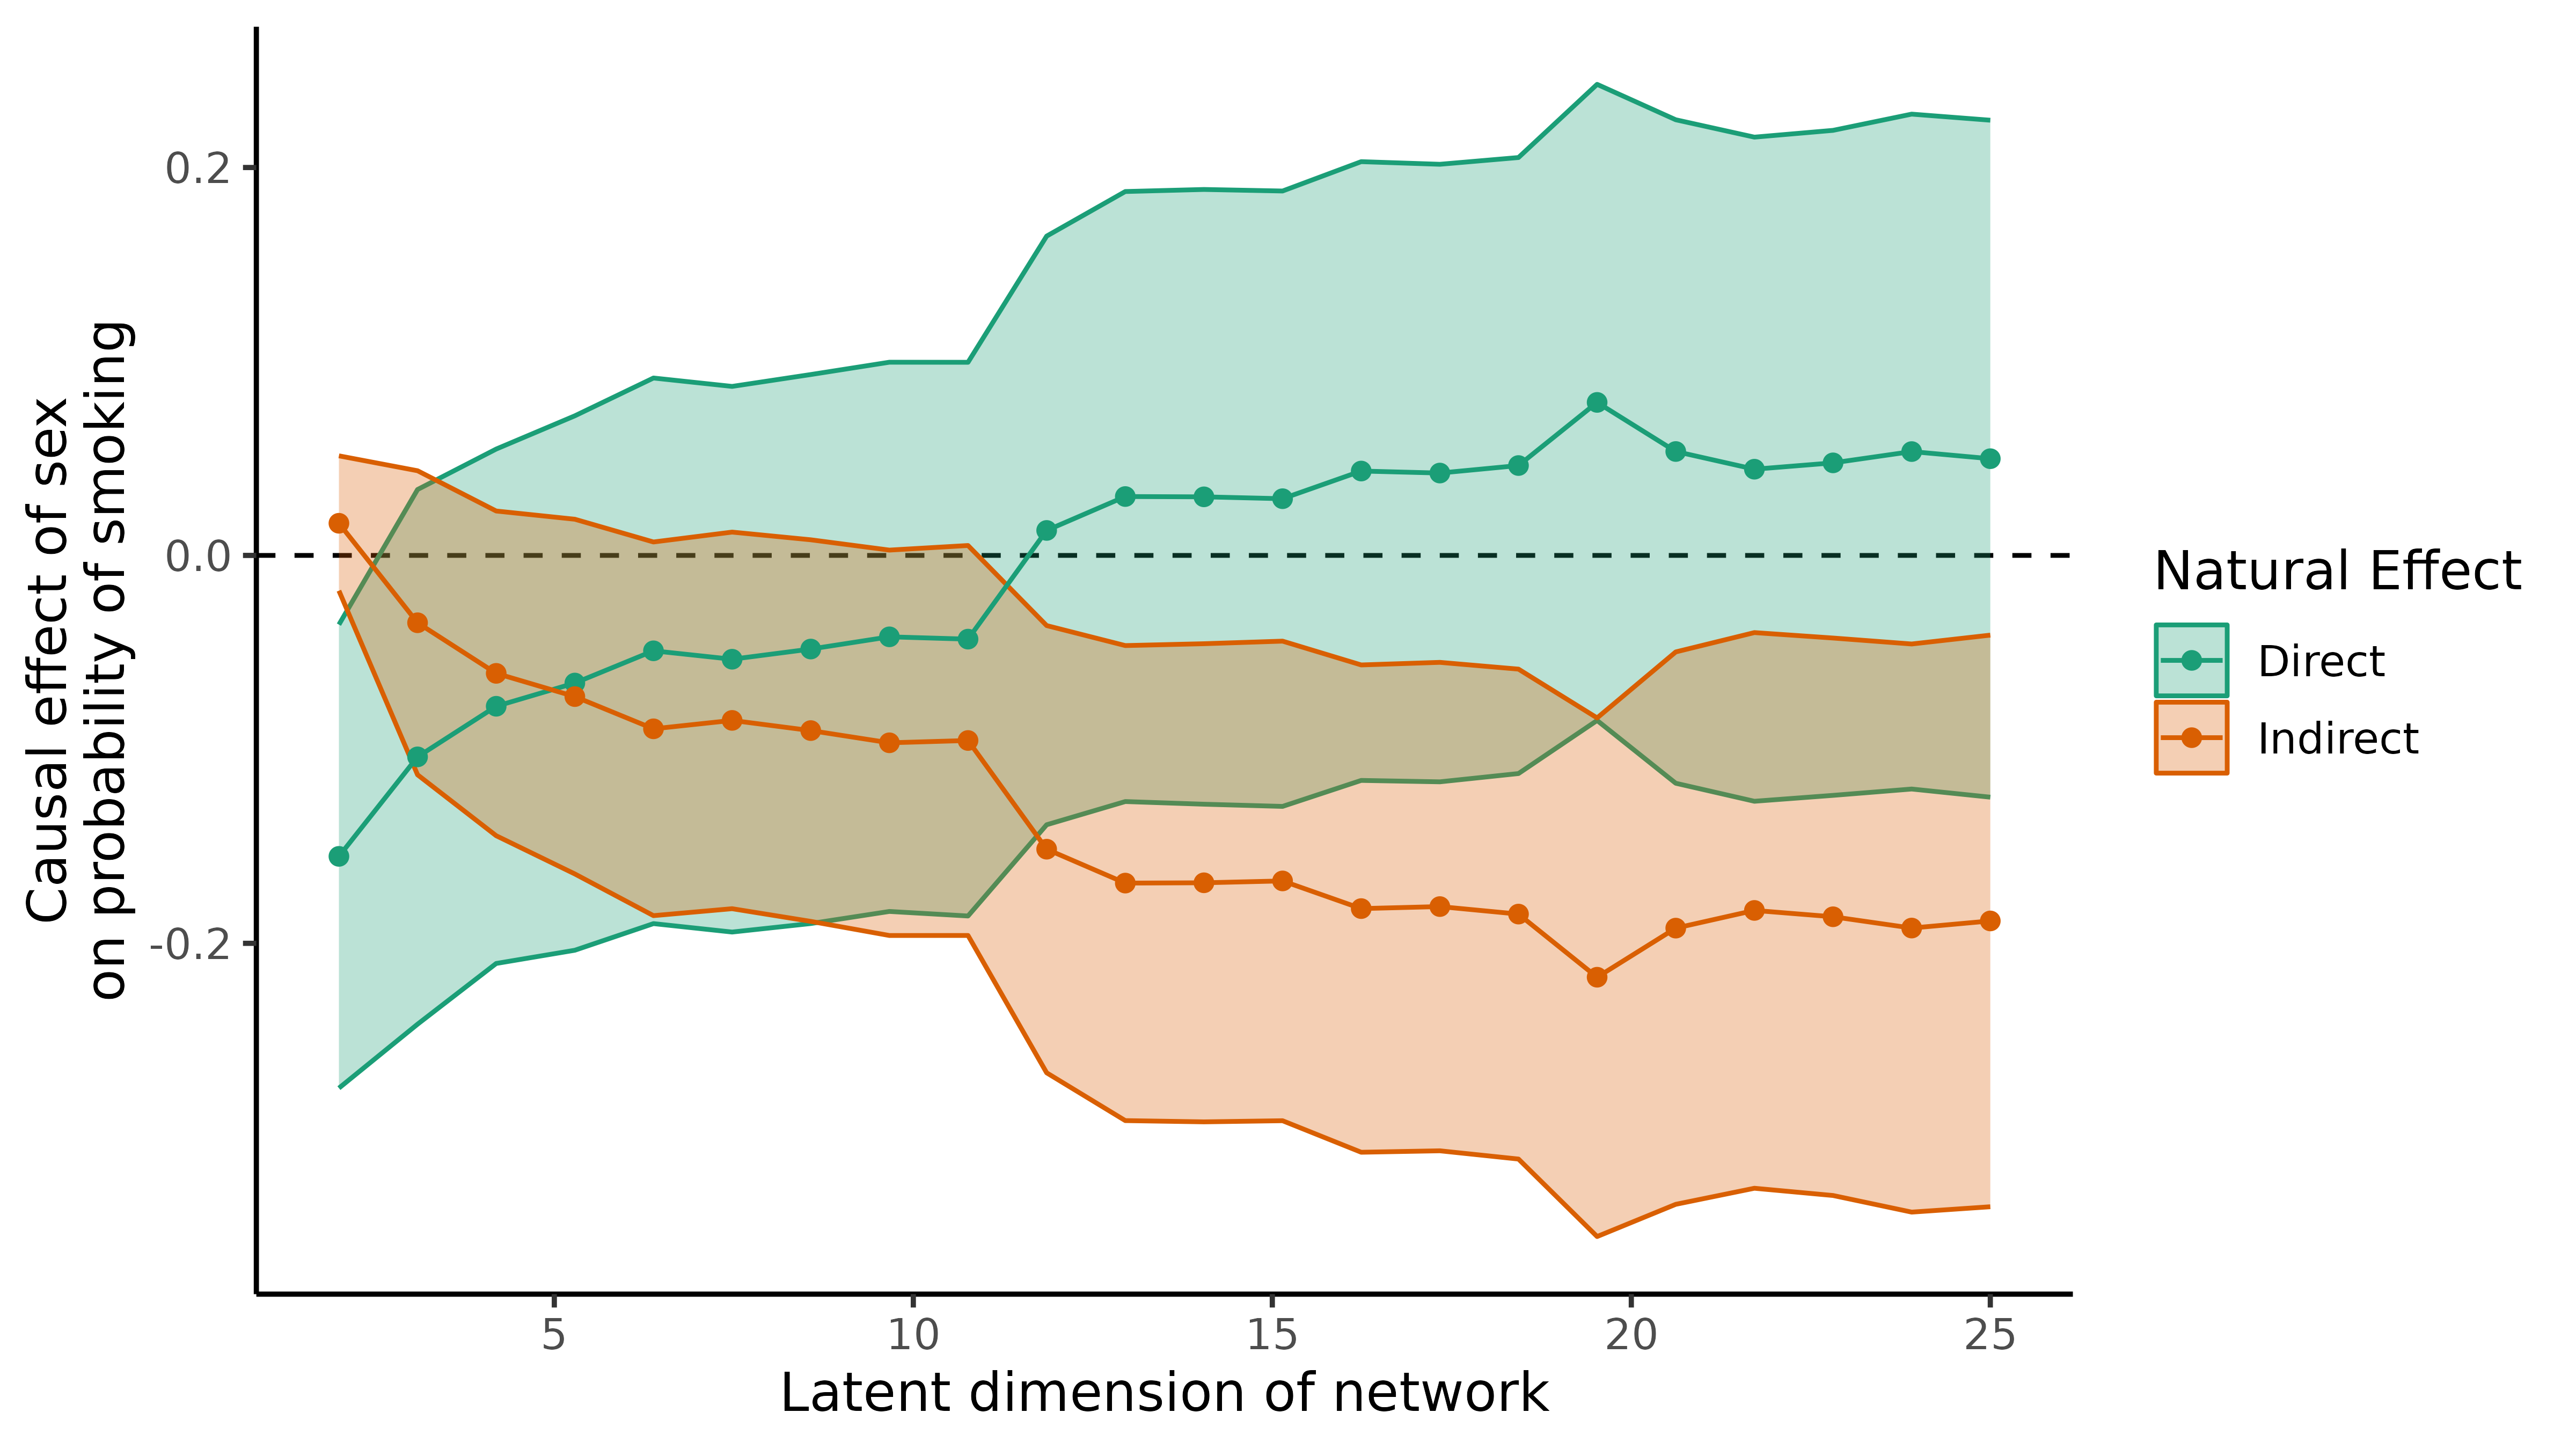
\includegraphics[width=0.5\textwidth]{figures/glasgow/effects.png}
          \caption{Estimated direct and indirect effects of sex on tobacco usage in the Glasgow social network. The estimated effects vary with the dimension $d$ of the latent space, and are adjusted for possibly confounding by age and church attendance. Positive values indicate a greater propensity for adolescent boys to smoke, negative effects a greater propensity for adolescent girls to smoke.}
          \label{fig:glasgow-estimates}
        \end{figure}

      \end{block}

      % \begin{block}{References}

      %   This talk is based on a manuscript recently submitted to JRSS-B, available as a pre-print at https://arxiv.org/abs/2212.12041.

      %   \nocite{*}
      %   \footnotesize{\bibliographystyle{plain}\bibliography{poster}}

      % \end{block}

    \end{column}

    \separatorcolumn
  \end{columns}
\end{frame}

\end{document}
